
  %% term_paper.tex
  %% Copyright 2018 Johanan Idicula
  %
  % This work may be distributed and/or modified under the
  % conditions of the LaTeX Project Public License, either version 1.3
  % of this license or (at your option) any later version.
  % The latest version of this license is in
  %   http://www.latex-project.org/lppl.txt
  % and version 1.3 or later is part of all distributions of LaTeX
  % version 2005/12/01 or later.
  %
  % This work has the LPPL maintenance status `maintained'.
  %
  % The Current Maintainer of this work is Johanan Idicula.
  %
  % This work consists of the file term_paper.tex.


%%%%%%%%%%%%%%%%%%%%%%%%%%%%%%%%%%%%%%%%%%%%%%%%%%%%%%%%%%%%%%%%%%%%% 
% McGill Term Paper Template
%
% 
% This is a title page template which is used for articles & reports.
% 
% 
%%%%%%%%%%%%%%%%%%%%%%%%%%%%%%%%%%%%%%%%%%%%%%%%%%%%%%%%%%%%%%%%%%%%%%

\documentclass[titlepage,12pt]{article}
\usepackage[margin=1in]{geometry}
\usepackage[myheadings]{fullpage}
% Uncomment next 2 lines to use TeX Gyre Heros sans serif
% \usepackage{tgheros,tgtermes,tgcursor}
% \renewcommand{\familydefault}{\sfdefault}
\usepackage{fancyhdr}
\usepackage{graphicx, wrapfig, subcaption, setspace, booktabs, titling}
\usepackage[font=small, labelfont=bf]{caption}
\usepackage[parfill]{parskip} % Activate to begin paragraphs with an empty line rather than an indent
\usepackage[english]{babel}
\usepackage{sectsty}
\usepackage{lipsum}
\usepackage{siunitx}
\DeclareSIUnit\molar{\mole\per\cubic\deci\metre}
\DeclareSIUnit\Molar{M}
\usepackage{mhchem}
\usepackage{pdfpages}
\usepackage[nottoc,numbib]{tocbibind}
\usepackage{textcomp}
\usepackage
	[%
	bookmarks=true,         % show bookmarks bar?
	unicode=false,          % non-Latin characters in Acrobat's bookmarks
	pdftoolbar=true,        % show Acrobat's toolbar?
	pdfmenubar=true,        % show Acrobat's menu?
	pdffitwindow=false,     % window fit to page when opened
	pdfstartview={FitH},    % fits the width of the page to the window
	pdftitle={Term Paper Template},    % title
	pdfauthor={Johanan Idicula},     % author
	pdfsubject={},   % subject of the document
	pdfcreator={Johanan Idicula},   % creator of the document
	pdfproducer={Johanan Idicula}, % producer of the document
	pdfkeywords={template, example, latex}, % list of keywords
	pdfnewwindow=true,      % links in new PDF window
	colorlinks=true,       % false: boxed links; true: colored links
	linkcolor=cyan,          % color of internal links (change box color with linkbordercolor)
	citecolor=red,        % color of links to bibliography
	filecolor=magenta,      % color of file links
	urlcolor=blue ,          % color of external links
	pdftex=true,%
	]{hyperref}%
\usepackage[numbers]{natbib}
\doublespacing
\setcounter{tocdepth}{5}
\setcounter{secnumdepth}{5}


%----------------------------------------------------------------------------
% TITLE PAGE
%----------------------------------------------------------------------------

\begin{document}

\title{\textbf{\LaTeX{} Term Paper Template}}

\date{\today}
\author{
		Johanan Idicula \\
		\href{mailto:johanan.idicula@mail.mcgill.ca}{johanan.idicula@mail.mcgill.ca} \\
		\href{https://github.com/jidicula/latex_templates}{github.com/jidicula/latex\_templates}
		 }

\maketitle
%----------------------------------------------------------------------------
% HEADER & FOOTER
%----------------------------------------------------------------------------
\pagestyle{fancy}
\fancyhf{}
\setlength\headheight{15pt}
\fancyhead[R]{BAM Lab}
\fancyhead[L]{Johanan Idicula}
\fancyhead[C]{\thetitle}
\fancyfoot[C]{\thepage}
%----------------------------------------------------------------------------
% Section title formatting

%----------------------------------------------------------------------------

%----------------------------------------------------------------------------
% Table of contents
\tableofcontents
\newpage

%----------------------------------------------------------------------------

%----------------------------------------------------------------------------
% BODY
%----------------------------------------------------------------------------
\section{SI Units}

The package \texttt{siunitx} allows you to correctly use SI units (like degrees Celsius). You can do proper SI formatting with \texttt{\textbackslash SI\{1\}\{\textbackslash meter\}} to render as \SI{1}{\meter}. See \href{http://ctan.mirror.rafal.ca/macros/latex/contrib/siunitx/siunitx.pdf}{the siunitx documentation} for more details. I've also included the molar symbol as a special command: \texttt{\textbackslash SI\{1\}\{\textbackslash Molar\}} becomes \SI{1}{\Molar}.

\section{Chemical equations}

The package \texttt{mhchem} allows you to make chemical formula, like \ce{MgCl2}. The full documentation is available \href{ftp://www.ctan.org/tex-archive/macros/latex/contrib/mhchem/mhchem.pdf}{here}.

\section{Figures}
I've included a bunch of figure snippets at the end of the source for this file. The best practice is to organize your images in a \texttt{./img/} directory. You can then link to a figure by referencing the label in \verb|\ref{fig:figlabel}|. For example, we plate our cells on a soft silicone substrate embedded with fluorescent beads for traction force microscopy, shown in Figure \ref{fig:TFM}. You can read more about cross-referencing \href{https://en.wikibooks.org/wiki/LaTeX/Labels_and_Cross-referencing}{here}.

\begin{figure}[!ht]
  \begin{center}
    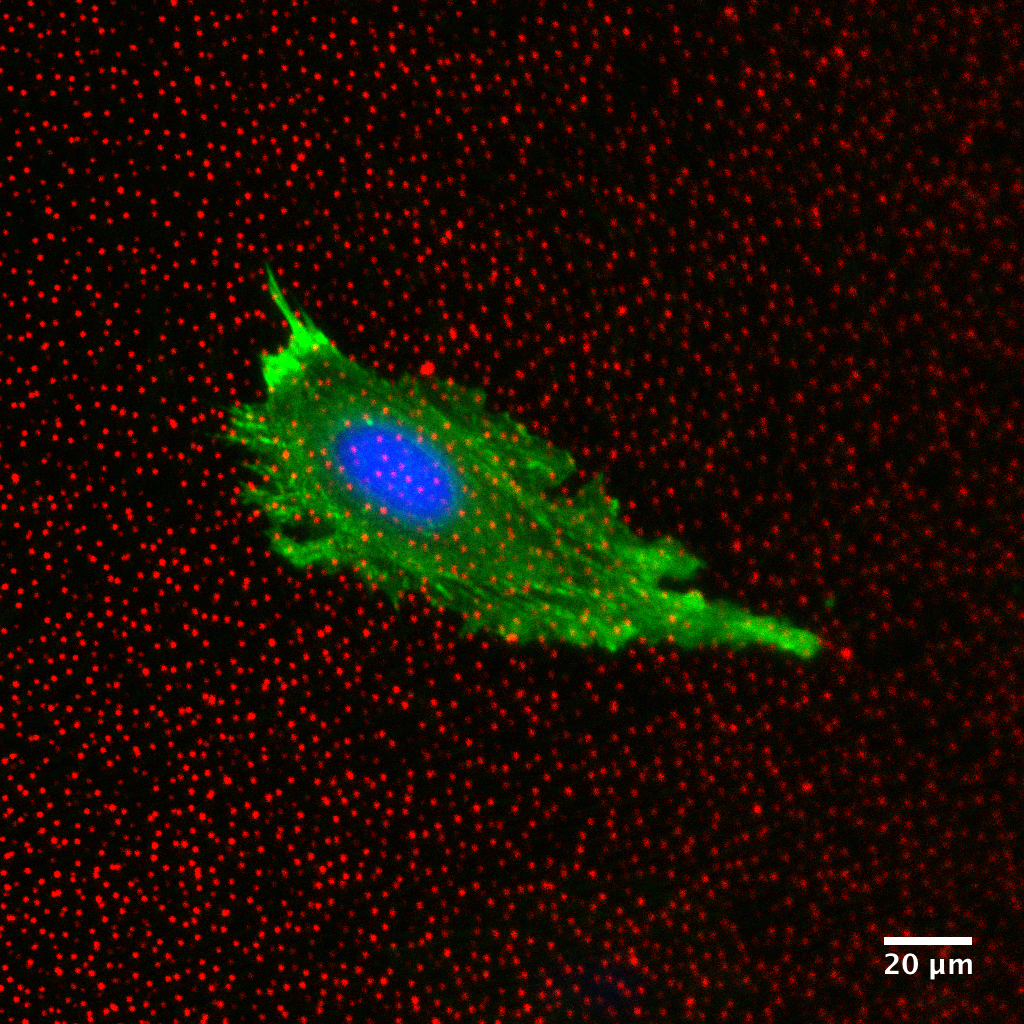
\includegraphics[width=0.29\textwidth]{img/Composite_scalebar_pos88}
  \end{center}
  \caption{HEK 293 cell transfected with ACTN4-hGFP and Nuc7-EBFP plated on a \SI{10}{\kilo\pascal} PDMS substrate embedded with a monolayer of poly methylmethacrylate DiI-core beads.}
  \label{fig:TFM}
\end{figure}

%\begin{wrapfigure}{r}{0.30\textwidth}
%	\vspace{-40pt}
%	\begin{center}
%		\includegraphics[width=0.29\textwidth]{file_name}
%	\end{center}
%	\vspace{-20pt}
%	\caption{}
%	\label{label:file_name}
%\end{wrapfigure}

\section{Citations}
You can easily cite sources using the cite keys for the entries in your \texttt{.bib} file. The bibliography styles are set and the bibliography is generated using
\begin{verbatim}
\bibliographystyle{unsrt}
\bibliography{term_paper}
\end{verbatim}

at location where you want your bibliography to be placed.

Here's an example:

My lab developed a technique for traction force microscopy on soft silicone substrates \cite{Yoshie:2018aa}. Deformation has been observed to be the independent variable in mechanotransduction \cite{Tajik_2016,Ehrlicher_2015}.

\bibliographystyle{unsrt}
\bibliography{term_paper}

\end{document}

%----------------------------------------------------------------------------
% SNIPPETS
%----------------------------------------------------------------------------

%\begin{figure}[!ht]
%	\centering
%	\includegraphics[width=0.8\textwidth]{file_name}
%	\caption{}
%	\centering
%	\label{label:file_name}
%\end{figure}

%\begin{figure}[!ht]
%	\centering
%	\includegraphics[width=0.8\textwidth]{graph}
%	\caption{Blood pressure ranges and associated level of hypertension (American Heart Association, 2013).}
%	\centering
%	\label{label:graph}
%\end{figure}

%\begin{wrapfigure}{r}{0.30\textwidth}
%	\vspace{-40pt}
%	\begin{center}
%		\includegraphics[width=0.29\textwidth]{file_name}
%	\end{center}
%	\vspace{-20pt}
%	\caption{}
%	\label{label:file_name}
%\end{wrapfigure}

%\begin{wrapfigure}{r}{0.45\textwidth}
%	\begin{center}
%		\includegraphics[width=0.29\textwidth]{manometer}
%	\end{center}
%	\caption{Aneroid sphygmomanometer with stethoscope (Medicalexpo, 2012).}
%	\label{label:manometer}
%\end{wrapfigure}

%\begin{table}[!ht]\footnotesize
%	\centering
%	\begin{tabular}{cccccc}
%	\toprule
%	\multicolumn{2}{c} {Pearson's correlation test} & \multicolumn{4}{c} {Independent t-test} \\
%	\midrule	
%	\multicolumn{2}{c} {Gender} & \multicolumn{2}{c} {Activity level} & \multicolumn{2}{c} {Gender} \\
%	\midrule
%	Males & Females & 1st level & 6th level & Males & Females \\
%	\midrule
%	\multicolumn{2}{c} {BMI vs. SP} & \multicolumn{2}{c} {Systolic pressure} & \multicolumn{2}{c} {Systolic Pressure} \\
%	\multicolumn{2}{c} {BMI vs. DP} & \multicolumn{2}{c} {Diastolic pressure} & \multicolumn{2}{c} {Diastolic pressure} \\
%	\multicolumn{2}{c} {BMI vs. MAP} & \multicolumn{2}{c} {MAP} & \multicolumn{2}{c} {MAP} \\
%	\multicolumn{2}{c} {W:H ratio vs. SP} & \multicolumn{2}{c} {BMI} & \multicolumn{2}{c} {BMI} \\
%	\multicolumn{2}{c} {W:H ratio vs. DP} & \multicolumn{2}{c} {W:H ratio} & \multicolumn{2}{c} {W:H ratio} \\
%	\multicolumn{2}{c} {W:H ratio vs. MAP} & \multicolumn{2}{c} {\% Body fat} & \multicolumn{2}{c} {\% Body fat} \\
%	\multicolumn{2}{c} {} & \multicolumn{2}{c} {Height} & \multicolumn{2}{c} {Height} \\
%	\multicolumn{2}{c} {} & \multicolumn{2}{c} {Weight} & \multicolumn{2}{c} {Weight} \\
%	\multicolumn{2}{c} {} & \multicolumn{2}{c} {Heart rate} & \multicolumn{2}{c} {Heart rate} \\
%	\bottomrule
%	\end{tabular}
%	\caption{Parameters that were analysed and related statistical test performed for current study. BMI - body mass index; SP - systolic pressure; DP - diastolic pressure; MAP - mean arterial pressure; W:H ratio - waist to hip ratio.}
%	\label{label:tests}
%\end{table}
